\documentclass[1p]{elsarticle_modified}
%\bibliographystyle{elsarticle-num}

%\usepackage[colorlinks]{hyperref}
%\usepackage{abbrmath_seonhwa} %\Abb, \Ascr, \Acal ,\Abf, \Afrak
\usepackage{amsfonts}
\usepackage{amssymb}
\usepackage{amsmath}
\usepackage{amsthm}
\usepackage{scalefnt}
\usepackage{amsbsy}
\usepackage{kotex}
\usepackage{caption}
\usepackage{subfig}
\usepackage{color}
\usepackage{graphicx}
\usepackage{xcolor} %% white, black, red, green, blue, cyan, magenta, yellow
\usepackage{float}
\usepackage{setspace}
\usepackage{hyperref}

\usepackage{tikz}
\usetikzlibrary{arrows}

\usepackage{multirow}
\usepackage{array} % fixed length table
\usepackage{hhline}

%%%%%%%%%%%%%%%%%%%%%
\makeatletter
\renewcommand*\env@matrix[1][\arraystretch]{%
	\edef\arraystretch{#1}%
	\hskip -\arraycolsep
	\let\@ifnextchar\new@ifnextchar
	\array{*\c@MaxMatrixCols c}}
\makeatother %https://tex.stackexchange.com/questions/14071/how-can-i-increase-the-line-spacing-in-a-matrix
%%%%%%%%%%%%%%%

\usepackage[normalem]{ulem}

\newcommand{\msout}[1]{\ifmmode\text{\sout{\ensuremath{#1}}}\else\sout{#1}\fi}
%SOURCE: \msout is \stkout macro in https://tex.stackexchange.com/questions/20609/strikeout-in-math-mode

\newcommand{\cancel}[1]{
	\ifmmode
	{\color{red}\msout{#1}}
	\else
	{\color{red}\sout{#1}}
	\fi
}

\newcommand{\add}[1]{
	{\color{blue}\uwave{#1}}
}

\newcommand{\replace}[2]{
	\ifmmode
	{\color{red}\msout{#1}}{\color{blue}\uwave{#2}}
	\else
	{\color{red}\sout{#1}}{\color{blue}\uwave{#2}}
	\fi
}

\newcommand{\Sol}{\mathcal{S}} %segment
\newcommand{\D}{D} %diagram
\newcommand{\A}{\mathcal{A}} %arc


%%%%%%%%%%%%%%%%%%%%%%%%%%%%%5 test

\def\sl{\operatorname{\textup{SL}}(2,\Cbb)}
\def\psl{\operatorname{\textup{PSL}}(2,\Cbb)}
\def\quan{\mkern 1mu \triangleright \mkern 1mu}

\theoremstyle{definition}
\newtheorem{thm}{Theorem}[section]
\newtheorem{prop}[thm]{Proposition}
\newtheorem{lem}[thm]{Lemma}
\newtheorem{ques}[thm]{Question}
\newtheorem{cor}[thm]{Corollary}
\newtheorem{defn}[thm]{Definition}
\newtheorem{exam}[thm]{Example}
\newtheorem{rmk}[thm]{Remark}
\newtheorem{alg}[thm]{Algorithm}

\newcommand{\I}{\sqrt{-1}}
\begin{document}

%\begin{frontmatter}
%
%\title{Boundary parabolic representations of knots up to 8 crossings}
%
%%% Group authors per affiliation:
%\author{Yunhi Cho} 
%\address{Department of Mathematics, University of Seoul, Seoul, Korea}
%\ead{yhcho@uos.ac.kr}
%
%
%\author{Seonhwa Kim} %\fnref{s_kim}}
%\address{Center for Geometry and Physics, Institute for Basic Science, Pohang, 37673, Korea}
%\ead{ryeona17@ibs.re.kr}
%
%\author{Hyuk Kim}
%\address{Department of Mathematical Sciences, Seoul National University, Seoul 08826, Korea}
%\ead{hyukkim@snu.ac.kr}
%
%\author{Seokbeom Yoon}
%\address{Department of Mathematical Sciences, Seoul National University, Seoul, 08826,  Korea}
%\ead{sbyoon15@snu.ac.kr}
%
%\begin{abstract}
%We find all boundary parabolic representation of knots up to 8 crossings.
%
%\end{abstract}
%\begin{keyword}
%    \MSC[2010] 57M25 
%\end{keyword}
%
%\end{frontmatter}

%\linenumbers
%\tableofcontents
%
\newcommand\colored[1]{\textcolor{white}{\rule[-0.35ex]{0.8em}{1.4ex}}\kern-0.8em\color{red} #1}%
%\newcommand\colored[1]{\textcolor{white}{ #1}\kern-2.17ex	\textcolor{white}{ #1}\kern-1.81ex	\textcolor{white}{ #1}\kern-2.15ex\color{red}#1	}

{\Large $\underline{12n_{0075}~(K12n_{0075})}$}

\setlength{\tabcolsep}{10pt}
\renewcommand{\arraystretch}{1.6}
\vspace{1cm}\begin{tabular}{m{100pt}>{\centering\arraybackslash}m{274pt}}
\multirow{5}{120pt}{
	\centering
	\includegraphics[width=112pt]{../../../GIT/diagram.site/Diagrams/png/2164_12n_0075.png}\\
\ \ \ A knot diagram\footnotemark}&
\allowdisplaybreaks
\textbf{Linearized knot diagam} \\
\cline{2-2}
 &
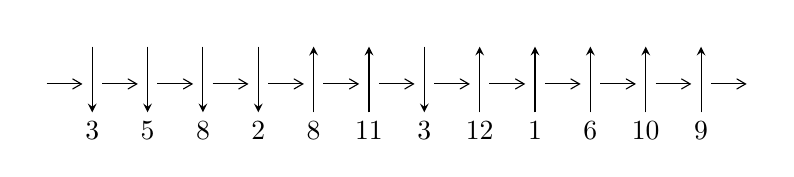
\begin{tikzpicture}[x=20pt, y=17pt]
	% nodes
	\node (C0) at (0, 0) {};
	\node (C1) at (1, 0) {};
	\node (C1U) at (1, +1) {};
	\node (C1D) at (1, -1) {3};

	\node (C2) at (2, 0) {};
	\node (C2U) at (2, +1) {};
	\node (C2D) at (2, -1) {5};

	\node (C3) at (3, 0) {};
	\node (C3U) at (3, +1) {};
	\node (C3D) at (3, -1) {8};

	\node (C4) at (4, 0) {};
	\node (C4U) at (4, +1) {};
	\node (C4D) at (4, -1) {2};

	\node (C5) at (5, 0) {};
	\node (C5U) at (5, +1) {};
	\node (C5D) at (5, -1) {8};

	\node (C6) at (6, 0) {};
	\node (C6U) at (6, +1) {};
	\node (C6D) at (6, -1) {11};

	\node (C7) at (7, 0) {};
	\node (C7U) at (7, +1) {};
	\node (C7D) at (7, -1) {3};

	\node (C8) at (8, 0) {};
	\node (C8U) at (8, +1) {};
	\node (C8D) at (8, -1) {12};

	\node (C9) at (9, 0) {};
	\node (C9U) at (9, +1) {};
	\node (C9D) at (9, -1) {1};

	\node (C10) at (10, 0) {};
	\node (C10U) at (10, +1) {};
	\node (C10D) at (10, -1) {6};

	\node (C11) at (11, 0) {};
	\node (C11U) at (11, +1) {};
	\node (C11D) at (11, -1) {10};

	\node (C12) at (12, 0) {};
	\node (C12U) at (12, +1) {};
	\node (C12D) at (12, -1) {9};
	\node (C13) at (13, 0) {};

	% arrows
	\draw[->,>={angle 60}]
	(C0) edge (C1) (C1) edge (C2) (C2) edge (C3) (C3) edge (C4) (C4) edge (C5) (C5) edge (C6) (C6) edge (C7) (C7) edge (C8) (C8) edge (C9) (C9) edge (C10) (C10) edge (C11) (C11) edge (C12) (C12) edge (C13) ;	\draw[->,>=stealth]
	(C1U) edge (C1D) (C2U) edge (C2D) (C3U) edge (C3D) (C4U) edge (C4D) (C5D) edge (C5U) (C6D) edge (C6U) (C7U) edge (C7D) (C8D) edge (C8U) (C9D) edge (C9U) (C10D) edge (C10U) (C11D) edge (C11U) (C12D) edge (C12U) ;
	\end{tikzpicture} \\
\hhline{~~} \\& 
\textbf{Solving Sequence} \\ \cline{2-2} 
 &
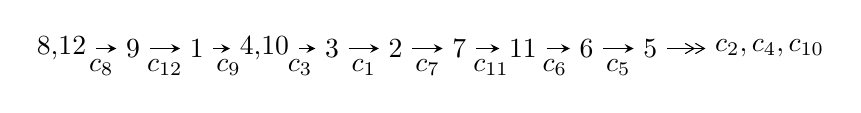
\begin{tikzpicture}[x=23pt, y=7pt]
	% node
	\node (A0) at (-1/8, 0) {8,12};
	\node (A1) at (1, 0) {9};
	\node (A2) at (2, 0) {1};
	\node (A3) at (49/16, 0) {4,10};
	\node (A4) at (33/8, 0) {3};
	\node (A5) at (41/8, 0) {2};
	\node (A6) at (49/8, 0) {7};
	\node (A7) at (57/8, 0) {11};
	\node (A8) at (65/8, 0) {6};
	\node (A9) at (73/8, 0) {5};
	\node (C1) at (1/2, -1) {$c_{8}$};
	\node (C2) at (3/2, -1) {$c_{12}$};
	\node (C3) at (5/2, -1) {$c_{9}$};
	\node (C4) at (29/8, -1) {$c_{3}$};
	\node (C5) at (37/8, -1) {$c_{1}$};
	\node (C6) at (45/8, -1) {$c_{7}$};
	\node (C7) at (53/8, -1) {$c_{11}$};
	\node (C8) at (61/8, -1) {$c_{6}$};
	\node (C9) at (69/8, -1) {$c_{5}$};
	\node (A10) at (11, 0) {$c_{2},c_{4},c_{10}$};

	% edge
	\draw[->,>=stealth]	
	(A0) edge (A1) (A1) edge (A2) (A2) edge (A3) (A3) edge (A4) (A4) edge (A5) (A5) edge (A6) (A6) edge (A7) (A7) edge (A8) (A8) edge (A9) ;
	\draw[->>,>={angle 60}]	
	(A9) edge (A10);
\end{tikzpicture} \\ 

\end{tabular} \\

\footnotetext{
The image of knot diagram is generated by the software ``\textbf{Draw programme}" developed by Andrew Bartholomew(\url{http://www.layer8.co.uk/maths/draw/index.htm\#Running-draw}), where we modified some parts for our purpose(\url{https://github.com/CATsTAILs/LinksPainter}).
}\phantom \\ \newline 
\centering \textbf{Ideals for irreducible components\footnotemark of $X_{\text{par}}$} 
 
\begin{align*}
I^u_{1}&=\langle 
-4.17318\times10^{15} u^{51}+1.53597\times10^{16} u^{50}+\cdots+1.39326\times10^{15} b+3.61251\times10^{15},\\
\phantom{I^u_{1}}&\phantom{= \langle  }3.45613\times10^{16} u^{51}-1.28036\times10^{17} u^{50}+\cdots+2.78652\times10^{15} a+6.93027\times10^{15},\;u^{52}-5 u^{51}+\cdots+14 u+1\rangle \\
I^u_{2}&=\langle 
b,\;u^7-2 u^6-2 u^5+4 u^4+2 u^3- u^2+a- u-3,\;u^8- u^7-3 u^6+2 u^5+3 u^4-2 u-1\rangle \\
I^u_{3}&=\langle 
a^2+5 b+3 a+5,\;a^3+a^2+4 a+5,\;u+1\rangle \\
\\
\end{align*}
\raggedright * 3 irreducible components of $\dim_{\mathbb{C}}=0$, with total 63 representations.\\
\footnotetext{All coefficients of polynomials are rational numbers. But the coefficients are sometimes approximated in decimal forms when there is not enough margin.}
\newpage
\renewcommand{\arraystretch}{1}
\centering \section*{I. $I^u_{1}= \langle -4.17\times10^{15} u^{51}+1.54\times10^{16} u^{50}+\cdots+1.39\times10^{15} b+3.61\times10^{15},\;3.46\times10^{16} u^{51}-1.28\times10^{17} u^{50}+\cdots+2.79\times10^{15} a+6.93\times10^{15},\;u^{52}-5 u^{51}+\cdots+14 u+1 \rangle$}
\flushleft \textbf{(i) Arc colorings}\\
\begin{tabular}{m{7pt} m{180pt} m{7pt} m{180pt} }
\flushright $a_{8}=$&$\begin{pmatrix}1\\0\end{pmatrix}$ \\
\flushright $a_{12}=$&$\begin{pmatrix}0\\u\end{pmatrix}$ \\
\flushright $a_{9}=$&$\begin{pmatrix}1\\- u^2\end{pmatrix}$ \\
\flushright $a_{1}=$&$\begin{pmatrix}u\\- u^3+u\end{pmatrix}$ \\
\flushright $a_{4}=$&$\begin{pmatrix}-12.4030 u^{51}+45.9484 u^{50}+\cdots+81.3098 u-2.48707\\2.99526 u^{51}-11.0243 u^{50}+\cdots-30.7361 u-2.59285\end{pmatrix}$ \\
\flushright $a_{10}=$&$\begin{pmatrix}- u^2+1\\u^4-2 u^2\end{pmatrix}$ \\
\flushright $a_{3}=$&$\begin{pmatrix}-9.40778 u^{51}+34.9242 u^{50}+\cdots+50.5737 u-5.07992\\2.99526 u^{51}-11.0243 u^{50}+\cdots-30.7361 u-2.59285\end{pmatrix}$ \\
\flushright $a_{2}=$&$\begin{pmatrix}17.4460 u^{51}-64.6564 u^{50}+\cdots-149.987 u-4.05564\\-3.75474 u^{51}+13.9757 u^{50}+\cdots+42.5139 u+3.15715\end{pmatrix}$ \\
\flushright $a_{7}=$&$\begin{pmatrix}-9.55271 u^{51}+35.8772 u^{50}+\cdots+88.4408 u+2.91964\\8.60172 u^{51}-33.2652 u^{50}+\cdots-104.422 u-7.28044\end{pmatrix}$ \\
\flushright $a_{11}=$&$\begin{pmatrix}- u^5+2 u^3- u\\u^7-3 u^5+2 u^3+u\end{pmatrix}$ \\
\flushright $a_{6}=$&$\begin{pmatrix}8.36062 u^{51}-30.6096 u^{50}+\cdots-105.182 u-10.2144\\3.75474 u^{51}-13.9757 u^{50}+\cdots-42.5139 u-3.15715\end{pmatrix}$ \\
\flushright $a_{5}=$&$\begin{pmatrix}4.60588 u^{51}-16.6339 u^{50}+\cdots-62.6681 u-7.05722\\3.75474 u^{51}-13.9757 u^{50}+\cdots-42.5139 u-3.15715\end{pmatrix}$\\&\end{tabular}
\flushleft \textbf{(ii) Obstruction class $= -1$}\\~\\
\flushleft \textbf{(iii) Cusp Shapes $= -\frac{11065552867124641}{1393259322402082} u^{51}+\frac{42789532669637567}{1393259322402082} u^{50}+\cdots+\frac{1199032770084567}{1393259322402082} u-\frac{7200606156302692}{696629661201041}$}\\~\\
\newpage\renewcommand{\arraystretch}{1}
\flushleft \textbf{(iv) u-Polynomials at the component}\newline \\
\begin{tabular}{m{50pt}|m{274pt}}
Crossings & \hspace{64pt}u-Polynomials at each crossing \\
\hline $$\begin{aligned}c_{1}\end{aligned}$$&$\begin{aligned}
&u^{52}+14 u^{51}+\cdots+43 u+1
\end{aligned}$\\
\hline $$\begin{aligned}c_{2},c_{4}\end{aligned}$$&$\begin{aligned}
&u^{52}-10 u^{51}+\cdots- u+1
\end{aligned}$\\
\hline $$\begin{aligned}c_{3},c_{7}\end{aligned}$$&$\begin{aligned}
&u^{52}-2 u^{51}+\cdots+384 u-256
\end{aligned}$\\
\hline $$\begin{aligned}c_{5}\end{aligned}$$&$\begin{aligned}
&u^{52}+3 u^{51}+\cdots- u-1
\end{aligned}$\\
\hline $$\begin{aligned}c_{6},c_{10}\end{aligned}$$&$\begin{aligned}
&u^{52}+2 u^{51}+\cdots-28 u-8
\end{aligned}$\\
\hline $$\begin{aligned}c_{8},c_{9},c_{12}\end{aligned}$$&$\begin{aligned}
&u^{52}+5 u^{51}+\cdots-14 u+1
\end{aligned}$\\
\hline $$\begin{aligned}c_{11}\end{aligned}$$&$\begin{aligned}
&u^{52}-24 u^{51}+\cdots-1488 u+64
\end{aligned}$\\
\hline
\end{tabular}\\~\\
\newpage\renewcommand{\arraystretch}{1}
\flushleft \textbf{(v) Riley Polynomials at the component}\newline \\
\begin{tabular}{m{50pt}|m{274pt}}
Crossings & \hspace{64pt}Riley Polynomials at each crossing \\
\hline $$\begin{aligned}c_{1}\end{aligned}$$&$\begin{aligned}
&y^{52}+58 y^{51}+\cdots-447 y+1
\end{aligned}$\\
\hline $$\begin{aligned}c_{2},c_{4}\end{aligned}$$&$\begin{aligned}
&y^{52}-14 y^{51}+\cdots-43 y+1
\end{aligned}$\\
\hline $$\begin{aligned}c_{3},c_{7}\end{aligned}$$&$\begin{aligned}
&y^{52}+54 y^{51}+\cdots+606208 y+65536
\end{aligned}$\\
\hline $$\begin{aligned}c_{5}\end{aligned}$$&$\begin{aligned}
&y^{52}-61 y^{51}+\cdots-19 y+1
\end{aligned}$\\
\hline $$\begin{aligned}c_{6},c_{10}\end{aligned}$$&$\begin{aligned}
&y^{52}-24 y^{51}+\cdots-1488 y+64
\end{aligned}$\\
\hline $$\begin{aligned}c_{8},c_{9},c_{12}\end{aligned}$$&$\begin{aligned}
&y^{52}-47 y^{51}+\cdots-104 y+1
\end{aligned}$\\
\hline $$\begin{aligned}c_{11}\end{aligned}$$&$\begin{aligned}
&y^{52}+4 y^{51}+\cdots-498944 y+4096
\end{aligned}$\\
\hline
\end{tabular}\\~\\
\newpage\flushleft \textbf{(vi) Complex Volumes and Cusp Shapes}
$$\begin{array}{c|c|c}  
\text{Solutions to }I^u_{1}& \I (\text{vol} + \sqrt{-1}CS) & \text{Cusp shape}\\
 \hline 
\begin{aligned}
u &= -0.864111 + 0.613274 I \\
a &= \phantom{-}0.72971 - 2.28554 I \\
b &= \phantom{-}0.08277 + 1.65392 I\end{aligned}
 & \phantom{-}7.67792 - 2.14785 I & \phantom{-}7.33727 + 2.34757 I \\ \hline\begin{aligned}
u &= -0.864111 - 0.613274 I \\
a &= \phantom{-}0.72971 + 2.28554 I \\
b &= \phantom{-}0.08277 - 1.65392 I\end{aligned}
 & \phantom{-}7.67792 + 2.14785 I & \phantom{-}7.33727 - 2.34757 I \\ \hline\begin{aligned}
u &= -0.278369 + 0.886469 I \\
a &= \phantom{-}0.81489 - 1.68991 I \\
b &= \phantom{-}0.52357 + 1.58617 I\end{aligned}
 & \phantom{-}5.03572 - 9.87508 I & \phantom{-}3.10372 + 7.08066 I \\ \hline\begin{aligned}
u &= -0.278369 - 0.886469 I \\
a &= \phantom{-}0.81489 + 1.68991 I \\
b &= \phantom{-}0.52357 - 1.58617 I\end{aligned}
 & \phantom{-}5.03572 + 9.87508 I & \phantom{-}3.10372 - 7.08066 I \\ \hline\begin{aligned}
u &= -0.344404 + 0.851796 I \\
a &= -0.85095 + 1.66493 I \\
b &= -0.08288 - 1.66614 I\end{aligned}
 & \phantom{-}6.09934 - 2.94801 I & \phantom{-}4.84338 + 2.76292 I \\ \hline\begin{aligned}
u &= -0.344404 - 0.851796 I \\
a &= -0.85095 - 1.66493 I \\
b &= -0.08288 + 1.66614 I\end{aligned}
 & \phantom{-}6.09934 + 2.94801 I & \phantom{-}4.84338 - 2.76292 I \\ \hline\begin{aligned}
u &= -0.959966 + 0.581836 I \\
a &= -0.84889 + 2.03520 I \\
b &= \phantom{-}0.40253 - 1.60177 I\end{aligned}
 & \phantom{-}7.11104 + 4.74276 I & \phantom{-0.000000 } 0 \\ \hline\begin{aligned}
u &= -0.959966 - 0.581836 I \\
a &= -0.84889 - 2.03520 I \\
b &= \phantom{-}0.40253 + 1.60177 I\end{aligned}
 & \phantom{-}7.11104 - 4.74276 I & \phantom{-0.000000 } 0 \\ \hline\begin{aligned}
u &= -1.149080 + 0.112159 I \\
a &= -0.11168 + 3.35174 I \\
b &= \phantom{-}0.257735 - 0.531872 I\end{aligned}
 & \phantom{-}0.064366 - 0.675431 I & \phantom{-0.000000 } 0 \\ \hline\begin{aligned}
u &= -1.149080 - 0.112159 I \\
a &= -0.11168 - 3.35174 I \\
b &= \phantom{-}0.257735 + 0.531872 I\end{aligned}
 & \phantom{-}0.064366 + 0.675431 I & \phantom{-0.000000 } 0\\
 \hline 
 \end{array}$$\newpage$$\begin{array}{c|c|c}  
\text{Solutions to }I^u_{1}& \I (\text{vol} + \sqrt{-1}CS) & \text{Cusp shape}\\
 \hline 
\begin{aligned}
u &= -0.078334 + 0.779627 I \\
a &= -0.0018202 - 0.0329755 I \\
b &= -0.000332 - 0.629614 I\end{aligned}
 & -2.90851 - 2.74298 I & \phantom{-}4.20673 + 3.96739 I \\ \hline\begin{aligned}
u &= -0.078334 - 0.779627 I \\
a &= -0.0018202 + 0.0329755 I \\
b &= -0.000332 + 0.629614 I\end{aligned}
 & -2.90851 + 2.74298 I & \phantom{-}4.20673 - 3.96739 I \\ \hline\begin{aligned}
u &= \phantom{-}1.219950 + 0.081401 I \\
a &= \phantom{-}0.28979 + 1.63338 I \\
b &= -0.347717 - 1.160600 I\end{aligned}
 & \phantom{-}5.43256 - 2.37277 I & \phantom{-0.000000 } 0 \\ \hline\begin{aligned}
u &= \phantom{-}1.219950 - 0.081401 I \\
a &= \phantom{-}0.28979 - 1.63338 I \\
b &= -0.347717 + 1.160600 I\end{aligned}
 & \phantom{-}5.43256 + 2.37277 I & \phantom{-0.000000 } 0 \\ \hline\begin{aligned}
u &= -0.282889 + 0.711805 I \\
a &= \phantom{-}0.178611 - 0.588706 I \\
b &= \phantom{-}1.029030 + 0.101314 I\end{aligned}
 & -0.42821 - 3.83727 I & \phantom{-}2.28173 + 6.95386 I \\ \hline\begin{aligned}
u &= -0.282889 - 0.711805 I \\
a &= \phantom{-}0.178611 + 0.588706 I \\
b &= \phantom{-}1.029030 - 0.101314 I\end{aligned}
 & -0.42821 + 3.83727 I & \phantom{-}2.28173 - 6.95386 I \\ \hline\begin{aligned}
u &= -1.193430 + 0.324240 I \\
a &= \phantom{-}0.669986 - 0.648263 I \\
b &= -0.015350 + 0.613459 I\end{aligned}
 & \phantom{-}0.485168 - 1.259080 I & \phantom{-0.000000 } 0 \\ \hline\begin{aligned}
u &= -1.193430 - 0.324240 I \\
a &= \phantom{-}0.669986 + 0.648263 I \\
b &= -0.015350 - 0.613459 I\end{aligned}
 & \phantom{-}0.485168 + 1.259080 I & \phantom{-0.000000 } 0 \\ \hline\begin{aligned}
u &= -0.680369 + 0.289746 I \\
a &= \phantom{-}0.012168 - 0.147432 I \\
b &= \phantom{-}0.638639 - 0.199115 I\end{aligned}
 & \phantom{-}1.074090 + 0.016258 I & \phantom{-}8.77032 - 1.10969 I \\ \hline\begin{aligned}
u &= -0.680369 - 0.289746 I \\
a &= \phantom{-}0.012168 + 0.147432 I \\
b &= \phantom{-}0.638639 + 0.199115 I\end{aligned}
 & \phantom{-}1.074090 - 0.016258 I & \phantom{-}8.77032 + 1.10969 I\\
 \hline 
 \end{array}$$\newpage$$\begin{array}{c|c|c}  
\text{Solutions to }I^u_{1}& \I (\text{vol} + \sqrt{-1}CS) & \text{Cusp shape}\\
 \hline 
\begin{aligned}
u &= -1.280180 + 0.138912 I \\
a &= \phantom{-}1.48485 + 1.45215 I \\
b &= -0.906569 - 0.186892 I\end{aligned}
 & \phantom{-}2.21484 - 2.00952 I & \phantom{-0.000000 } 0 \\ \hline\begin{aligned}
u &= -1.280180 - 0.138912 I \\
a &= \phantom{-}1.48485 - 1.45215 I \\
b &= -0.906569 + 0.186892 I\end{aligned}
 & \phantom{-}2.21484 + 2.00952 I & \phantom{-0.000000 } 0 \\ \hline\begin{aligned}
u &= -0.710230\phantom{ +0.000000I} \\
a &= \phantom{-}0.329379\phantom{ +0.000000I} \\
b &= \phantom{-}0.453636\phantom{ +0.000000I}\end{aligned}
 & \phantom{-}1.01816\phantom{ +0.000000I} & \phantom{-}10.6560\phantom{ +0.000000I} \\ \hline\begin{aligned}
u &= -0.202574 + 0.614660 I \\
a &= -0.41637 - 1.80557 I \\
b &= -0.212659 + 0.790964 I\end{aligned}
 & -2.49821 - 1.98647 I & \phantom{-}1.56783 + 2.89756 I \\ \hline\begin{aligned}
u &= -0.202574 - 0.614660 I \\
a &= -0.41637 + 1.80557 I \\
b &= -0.212659 - 0.790964 I\end{aligned}
 & -2.49821 + 1.98647 I & \phantom{-}1.56783 - 2.89756 I \\ \hline\begin{aligned}
u &= \phantom{-}1.316330 + 0.333742 I \\
a &= -0.408950 - 0.703118 I \\
b &= -0.036069 + 0.646778 I\end{aligned}
 & \phantom{-}1.46111 + 6.76040 I & \phantom{-0.000000 } 0 \\ \hline\begin{aligned}
u &= \phantom{-}1.316330 - 0.333742 I \\
a &= -0.408950 + 0.703118 I \\
b &= -0.036069 - 0.646778 I\end{aligned}
 & \phantom{-}1.46111 - 6.76040 I & \phantom{-0.000000 } 0 \\ \hline\begin{aligned}
u &= \phantom{-}0.240670 + 0.591040 I \\
a &= -1.50879 - 1.89532 I \\
b &= -0.38554 + 1.46577 I\end{aligned}
 & \phantom{-}2.88733 + 4.52304 I & -0.03636 - 3.32255 I \\ \hline\begin{aligned}
u &= \phantom{-}0.240670 - 0.591040 I \\
a &= -1.50879 + 1.89532 I \\
b &= -0.38554 - 1.46577 I\end{aligned}
 & \phantom{-}2.88733 - 4.52304 I & -0.03636 + 3.32255 I \\ \hline\begin{aligned}
u &= \phantom{-}1.371880 + 0.190150 I \\
a &= \phantom{-}0.51449 - 1.70845 I \\
b &= -0.965667 + 0.552199 I\end{aligned}
 & \phantom{-}3.35341 + 2.44910 I & \phantom{-0.000000 } 0\\
 \hline 
 \end{array}$$\newpage$$\begin{array}{c|c|c}  
\text{Solutions to }I^u_{1}& \I (\text{vol} + \sqrt{-1}CS) & \text{Cusp shape}\\
 \hline 
\begin{aligned}
u &= \phantom{-}1.371880 - 0.190150 I \\
a &= \phantom{-}0.51449 + 1.70845 I \\
b &= -0.965667 - 0.552199 I\end{aligned}
 & \phantom{-}3.35341 - 2.44910 I & \phantom{-0.000000 } 0 \\ \hline\begin{aligned}
u &= \phantom{-}1.381790 + 0.242632 I \\
a &= \phantom{-}0.70682 + 2.59552 I \\
b &= -0.377861 - 1.015230 I\end{aligned}
 & \phantom{-}2.55895 + 5.12601 I & \phantom{-0.000000 } 0 \\ \hline\begin{aligned}
u &= \phantom{-}1.381790 - 0.242632 I \\
a &= \phantom{-}0.70682 - 2.59552 I \\
b &= -0.377861 + 1.015230 I\end{aligned}
 & \phantom{-}2.55895 - 5.12601 I & \phantom{-0.000000 } 0 \\ \hline\begin{aligned}
u &= -1.39431 + 0.23988 I \\
a &= -0.79430 + 4.03936 I \\
b &= -0.47035 - 1.61370 I\end{aligned}
 & \phantom{-}8.11020 - 7.60143 I & \phantom{-0.000000 } 0 \\ \hline\begin{aligned}
u &= -1.39431 - 0.23988 I \\
a &= -0.79430 - 4.03936 I \\
b &= -0.47035 + 1.61370 I\end{aligned}
 & \phantom{-}8.11020 + 7.60143 I & \phantom{-0.000000 } 0 \\ \hline\begin{aligned}
u &= -1.40452 + 0.18151 I \\
a &= \phantom{-}1.20569 - 4.10928 I \\
b &= \phantom{-}0.00116 + 1.68427 I\end{aligned}
 & \phantom{-}8.93491 - 0.61807 I & \phantom{-0.000000 } 0 \\ \hline\begin{aligned}
u &= -1.40452 - 0.18151 I \\
a &= \phantom{-}1.20569 + 4.10928 I \\
b &= \phantom{-}0.00116 - 1.68427 I\end{aligned}
 & \phantom{-}8.93491 + 0.61807 I & \phantom{-0.000000 } 0 \\ \hline\begin{aligned}
u &= \phantom{-}1.42142 + 0.11111 I \\
a &= -1.39366 - 1.43200 I \\
b &= \phantom{-}0.813091 + 0.784592 I\end{aligned}
 & \phantom{-}7.33747 + 1.34403 I & \phantom{-0.000000 } 0 \\ \hline\begin{aligned}
u &= \phantom{-}1.42142 - 0.11111 I \\
a &= -1.39366 + 1.43200 I \\
b &= \phantom{-}0.813091 - 0.784592 I\end{aligned}
 & \phantom{-}7.33747 - 1.34403 I & \phantom{-0.000000 } 0 \\ \hline\begin{aligned}
u &= \phantom{-}1.41493 + 0.27859 I \\
a &= -1.41802 + 1.14138 I \\
b &= \phantom{-}1.235590 - 0.150942 I\end{aligned}
 & \phantom{-}4.99311 + 7.43624 I & \phantom{-0.000000 } 0\\
 \hline 
 \end{array}$$\newpage$$\begin{array}{c|c|c}  
\text{Solutions to }I^u_{1}& \I (\text{vol} + \sqrt{-1}CS) & \text{Cusp shape}\\
 \hline 
\begin{aligned}
u &= \phantom{-}1.41493 - 0.27859 I \\
a &= -1.41802 - 1.14138 I \\
b &= \phantom{-}1.235590 + 0.150942 I\end{aligned}
 & \phantom{-}4.99311 - 7.43624 I & \phantom{-0.000000 } 0 \\ \hline\begin{aligned}
u &= \phantom{-}0.314249 + 0.443599 I \\
a &= \phantom{-}1.74200 + 2.01299 I \\
b &= -0.08624 - 1.45158 I\end{aligned}
 & \phantom{-}3.45819 - 1.75596 I & \phantom{-}0.22172 + 1.56110 I \\ \hline\begin{aligned}
u &= \phantom{-}0.314249 - 0.443599 I \\
a &= \phantom{-}1.74200 - 2.01299 I \\
b &= -0.08624 + 1.45158 I\end{aligned}
 & \phantom{-}3.45819 + 1.75596 I & \phantom{-}0.22172 - 1.56110 I \\ \hline\begin{aligned}
u &= \phantom{-}1.43910 + 0.36041 I \\
a &= \phantom{-}0.67098 + 3.42215 I \\
b &= \phantom{-}0.61263 - 1.61586 I\end{aligned}
 & \phantom{-}10.5096 + 14.3678 I & \phantom{-0.000000 } 0 \\ \hline\begin{aligned}
u &= \phantom{-}1.43910 - 0.36041 I \\
a &= \phantom{-}0.67098 - 3.42215 I \\
b &= \phantom{-}0.61263 + 1.61586 I\end{aligned}
 & \phantom{-}10.5096 - 14.3678 I & \phantom{-0.000000 } 0 \\ \hline\begin{aligned}
u &= \phantom{-}1.46087 + 0.32708 I \\
a &= -1.00755 - 3.48031 I \\
b &= -0.19562 + 1.75720 I\end{aligned}
 & \phantom{-}11.89100 + 7.20080 I & \phantom{-0.000000 } 0 \\ \hline\begin{aligned}
u &= \phantom{-}1.46087 - 0.32708 I \\
a &= -1.00755 + 3.48031 I \\
b &= -0.19562 - 1.75720 I\end{aligned}
 & \phantom{-}11.89100 - 7.20080 I & \phantom{-0.000000 } 0 \\ \hline\begin{aligned}
u &= -0.111943 + 0.439985 I \\
a &= -1.241660 - 0.569711 I \\
b &= -0.772681 - 0.211532 I\end{aligned}
 & -1.51612 - 0.05304 I & -2.94270 + 1.44002 I \\ \hline\begin{aligned}
u &= -0.111943 - 0.439985 I \\
a &= -1.241660 + 0.569711 I \\
b &= -0.772681 + 0.211532 I\end{aligned}
 & -1.51612 + 0.05304 I & -2.94270 - 1.44002 I \\ \hline\begin{aligned}
u &= \phantom{-}1.54580 + 0.02807 I \\
a &= -0.26431 + 4.14163 I \\
b &= \phantom{-}0.27010 - 1.83700 I\end{aligned}
 & \phantom{-}16.1487 + 3.7905 I & \phantom{-0.000000 } 0\\
 \hline 
 \end{array}$$\newpage$$\begin{array}{c|c|c}  
\text{Solutions to }I^u_{1}& \I (\text{vol} + \sqrt{-1}CS) & \text{Cusp shape}\\
 \hline 
\begin{aligned}
u &= \phantom{-}1.54580 - 0.02807 I \\
a &= -0.26431 - 4.14163 I \\
b &= \phantom{-}0.27010 + 1.83700 I\end{aligned}
 & \phantom{-}16.1487 - 3.7905 I & \phantom{-0.000000 } 0 \\ \hline\begin{aligned}
u &= -0.0947755\phantom{ +0.000000I} \\
a &= -7.83548\phantom{ +0.000000I} \\
b &= -0.476249\phantom{ +0.000000I}\end{aligned}
 & -1.21791\phantom{ +0.000000I} & -10.0970\phantom{ +0.000000I}\\
 \hline 
 \end{array}$$\newpage\newpage\renewcommand{\arraystretch}{1}
\centering \section*{II. $I^u_{2}= \langle b,\;u^7-2 u^6-2 u^5+4 u^4+2 u^3- u^2+a- u-3,\;u^8- u^7-3 u^6+2 u^5+3 u^4-2 u-1 \rangle$}
\flushleft \textbf{(i) Arc colorings}\\
\begin{tabular}{m{7pt} m{180pt} m{7pt} m{180pt} }
\flushright $a_{8}=$&$\begin{pmatrix}1\\0\end{pmatrix}$ \\
\flushright $a_{12}=$&$\begin{pmatrix}0\\u\end{pmatrix}$ \\
\flushright $a_{9}=$&$\begin{pmatrix}1\\- u^2\end{pmatrix}$ \\
\flushright $a_{1}=$&$\begin{pmatrix}u\\- u^3+u\end{pmatrix}$ \\
\flushright $a_{4}=$&$\begin{pmatrix}- u^7+2 u^6+2 u^5-4 u^4-2 u^3+u^2+u+3\\0\end{pmatrix}$ \\
\flushright $a_{10}=$&$\begin{pmatrix}- u^2+1\\u^4-2 u^2\end{pmatrix}$ \\
\flushright $a_{3}=$&$\begin{pmatrix}- u^7+2 u^6+2 u^5-4 u^4-2 u^3+u^2+u+3\\0\end{pmatrix}$ \\
\flushright $a_{2}=$&$\begin{pmatrix}- u^7+2 u^6+2 u^5-4 u^4-2 u^3+u^2+2 u+3\\- u^3+u\end{pmatrix}$ \\
\flushright $a_{7}=$&$\begin{pmatrix}1\\0\end{pmatrix}$ \\
\flushright $a_{11}=$&$\begin{pmatrix}- u^5+2 u^3- u\\u^7-3 u^5+2 u^3+u\end{pmatrix}$ \\
\flushright $a_{6}=$&$\begin{pmatrix}u^3-2 u\\u^3- u\end{pmatrix}$ \\
\flushright $a_{5}=$&$\begin{pmatrix}- u\\u^3- u\end{pmatrix}$\\&\end{tabular}
\flushleft \textbf{(ii) Obstruction class $= 1$}\\~\\
\flushleft \textbf{(iii) Cusp Shapes $= -3 u^7+10 u^6+7 u^5-25 u^4-9 u^3+12 u^2+8 u+13$}\\~\\
\newpage\renewcommand{\arraystretch}{1}
\flushleft \textbf{(iv) u-Polynomials at the component}\newline \\
\begin{tabular}{m{50pt}|m{274pt}}
Crossings & \hspace{64pt}u-Polynomials at each crossing \\
\hline $$\begin{aligned}c_{1},c_{2}\end{aligned}$$&$\begin{aligned}
&(u-1)^8
\end{aligned}$\\
\hline $$\begin{aligned}c_{3},c_{7}\end{aligned}$$&$\begin{aligned}
&u^8
\end{aligned}$\\
\hline $$\begin{aligned}c_{4}\end{aligned}$$&$\begin{aligned}
&(u+1)^8
\end{aligned}$\\
\hline $$\begin{aligned}c_{5}\end{aligned}$$&$\begin{aligned}
&u^8+3 u^7+7 u^6+10 u^5+11 u^4+10 u^3+6 u^2+4 u+1
\end{aligned}$\\
\hline $$\begin{aligned}c_{6}\end{aligned}$$&$\begin{aligned}
&u^8+u^7- u^6-2 u^5+u^4+2 u^3-2 u-1
\end{aligned}$\\
\hline $$\begin{aligned}c_{8},c_{9}\end{aligned}$$&$\begin{aligned}
&u^8- u^7-3 u^6+2 u^5+3 u^4-2 u-1
\end{aligned}$\\
\hline $$\begin{aligned}c_{10}\end{aligned}$$&$\begin{aligned}
&u^8- u^7- u^6+2 u^5+u^4-2 u^3+2 u-1
\end{aligned}$\\
\hline $$\begin{aligned}c_{11}\end{aligned}$$&$\begin{aligned}
&u^8-3 u^7+7 u^6-10 u^5+11 u^4-10 u^3+6 u^2-4 u+1
\end{aligned}$\\
\hline $$\begin{aligned}c_{12}\end{aligned}$$&$\begin{aligned}
&u^8+u^7-3 u^6-2 u^5+3 u^4+2 u-1
\end{aligned}$\\
\hline
\end{tabular}\\~\\
\newpage\renewcommand{\arraystretch}{1}
\flushleft \textbf{(v) Riley Polynomials at the component}\newline \\
\begin{tabular}{m{50pt}|m{274pt}}
Crossings & \hspace{64pt}Riley Polynomials at each crossing \\
\hline $$\begin{aligned}c_{1},c_{2},c_{4}\end{aligned}$$&$\begin{aligned}
&(y-1)^8
\end{aligned}$\\
\hline $$\begin{aligned}c_{3},c_{7}\end{aligned}$$&$\begin{aligned}
&y^8
\end{aligned}$\\
\hline $$\begin{aligned}c_{5},c_{11}\end{aligned}$$&$\begin{aligned}
&y^8+5 y^7+11 y^6+6 y^5-17 y^4-34 y^3-22 y^2-4 y+1
\end{aligned}$\\
\hline $$\begin{aligned}c_{6},c_{10}\end{aligned}$$&$\begin{aligned}
&y^8-3 y^7+7 y^6-10 y^5+11 y^4-10 y^3+6 y^2-4 y+1
\end{aligned}$\\
\hline $$\begin{aligned}c_{8},c_{9},c_{12}\end{aligned}$$&$\begin{aligned}
&y^8-7 y^7+19 y^6-22 y^5+3 y^4+14 y^3-6 y^2-4 y+1
\end{aligned}$\\
\hline
\end{tabular}\\~\\
\newpage\flushleft \textbf{(vi) Complex Volumes and Cusp Shapes}
$$\begin{array}{c|c|c}  
\text{Solutions to }I^u_{2}& \I (\text{vol} + \sqrt{-1}CS) & \text{Cusp shape}\\
 \hline 
\begin{aligned}
u &= -1.180120 + 0.268597 I \\
a &= -0.281371 - 1.128550 I \\
b &= \phantom{-0.000000 } 0\end{aligned}
 & -0.604279 - 1.131230 I & -2.43193 + 0.79885 I \\ \hline\begin{aligned}
u &= -1.180120 - 0.268597 I \\
a &= -0.281371 + 1.128550 I \\
b &= \phantom{-0.000000 } 0\end{aligned}
 & -0.604279 + 1.131230 I & -2.43193 - 0.79885 I \\ \hline\begin{aligned}
u &= -0.108090 + 0.747508 I \\
a &= \phantom{-}0.208670 + 0.825203 I \\
b &= \phantom{-0.000000 } 0\end{aligned}
 & -3.80435 - 2.57849 I & -5.57469 + 3.25625 I \\ \hline\begin{aligned}
u &= -0.108090 - 0.747508 I \\
a &= \phantom{-}0.208670 - 0.825203 I \\
b &= \phantom{-0.000000 } 0\end{aligned}
 & -3.80435 + 2.57849 I & -5.57469 - 3.25625 I \\ \hline\begin{aligned}
u &= \phantom{-}1.37100\phantom{ +0.000000I} \\
a &= \phantom{-}0.829189\phantom{ +0.000000I} \\
b &= \phantom{-0.000000 } 0\end{aligned}
 & \phantom{-}4.85780\phantom{ +0.000000I} & \phantom{-}8.00600\phantom{ +0.000000I} \\ \hline\begin{aligned}
u &= \phantom{-}1.334530 + 0.318930 I \\
a &= \phantom{-}0.284386 - 0.605794 I \\
b &= \phantom{-0.000000 } 0\end{aligned}
 & \phantom{-}0.73474 + 6.44354 I & -0.28408 - 3.92092 I \\ \hline\begin{aligned}
u &= \phantom{-}1.334530 - 0.318930 I \\
a &= \phantom{-}0.284386 + 0.605794 I \\
b &= \phantom{-0.000000 } 0\end{aligned}
 & \phantom{-}0.73474 - 6.44354 I & -0.28408 + 3.92092 I \\ \hline\begin{aligned}
u &= -0.463640\phantom{ +0.000000I} \\
a &= \phantom{-}2.74744\phantom{ +0.000000I} \\
b &= \phantom{-0.000000 } 0\end{aligned}
 & -0.799899\phantom{ +0.000000I} & \phantom{-}11.5750\phantom{ +0.000000I}\\
 \hline 
 \end{array}$$\newpage\newpage\renewcommand{\arraystretch}{1}
\centering \section*{III. $I^u_{3}= \langle a^2+5 b+3 a+5,\;a^3+a^2+4 a+5,\;u+1 \rangle$}
\flushleft \textbf{(i) Arc colorings}\\
\begin{tabular}{m{7pt} m{180pt} m{7pt} m{180pt} }
\flushright $a_{8}=$&$\begin{pmatrix}1\\0\end{pmatrix}$ \\
\flushright $a_{12}=$&$\begin{pmatrix}0\\-1\end{pmatrix}$ \\
\flushright $a_{9}=$&$\begin{pmatrix}1\\-1\end{pmatrix}$ \\
\flushright $a_{1}=$&$\begin{pmatrix}-1\\0\end{pmatrix}$ \\
\flushright $a_{4}=$&$\begin{pmatrix}a\\-\frac{1}{5} a^2-\frac{3}{5} a-1\end{pmatrix}$ \\
\flushright $a_{10}=$&$\begin{pmatrix}0\\-1\end{pmatrix}$ \\
\flushright $a_{3}=$&$\begin{pmatrix}-\frac{1}{5} a^2+\frac{2}{5} a-1\\-\frac{1}{5} a^2-\frac{3}{5} a-1\end{pmatrix}$ \\
\flushright $a_{2}=$&$\begin{pmatrix}-2\\-\frac{2}{5} a^2-\frac{1}{5} a\end{pmatrix}$ \\
\flushright $a_{7}=$&$\begin{pmatrix}0\\-\frac{2}{5} a^2-\frac{1}{5} a\end{pmatrix}$ \\
\flushright $a_{11}=$&$\begin{pmatrix}0\\-1\end{pmatrix}$ \\
\flushright $a_{6}=$&$\begin{pmatrix}0\\-\frac{2}{5} a^2-\frac{1}{5} a\end{pmatrix}$ \\
\flushright $a_{5}=$&$\begin{pmatrix}\frac{2}{5} a^2+\frac{1}{5} a\\-\frac{2}{5} a^2-\frac{1}{5} a\end{pmatrix}$\\&\end{tabular}
\flushleft \textbf{(ii) Obstruction class $= 1$}\\~\\
\flushleft \textbf{(iii) Cusp Shapes $= -\frac{9}{5} a^2+\frac{13}{5} a-5$}\\~\\
\newpage\renewcommand{\arraystretch}{1}
\flushleft \textbf{(iv) u-Polynomials at the component}\newline \\
\begin{tabular}{m{50pt}|m{274pt}}
Crossings & \hspace{64pt}u-Polynomials at each crossing \\
\hline $$\begin{aligned}c_{1},c_{3}\end{aligned}$$&$\begin{aligned}
&u^3- u^2+2 u-1
\end{aligned}$\\
\hline $$\begin{aligned}c_{2}\end{aligned}$$&$\begin{aligned}
&u^3+u^2-1
\end{aligned}$\\
\hline $$\begin{aligned}c_{4}\end{aligned}$$&$\begin{aligned}
&u^3- u^2+1
\end{aligned}$\\
\hline $$\begin{aligned}c_{5}\end{aligned}$$&$\begin{aligned}
&u^3+3 u^2+2 u-1
\end{aligned}$\\
\hline $$\begin{aligned}c_{6},c_{10},c_{11}\end{aligned}$$&$\begin{aligned}
&u^3
\end{aligned}$\\
\hline $$\begin{aligned}c_{7}\end{aligned}$$&$\begin{aligned}
&u^3+u^2+2 u+1
\end{aligned}$\\
\hline $$\begin{aligned}c_{8},c_{9}\end{aligned}$$&$\begin{aligned}
&(u+1)^3
\end{aligned}$\\
\hline $$\begin{aligned}c_{12}\end{aligned}$$&$\begin{aligned}
&(u-1)^3
\end{aligned}$\\
\hline
\end{tabular}\\~\\
\newpage\renewcommand{\arraystretch}{1}
\flushleft \textbf{(v) Riley Polynomials at the component}\newline \\
\begin{tabular}{m{50pt}|m{274pt}}
Crossings & \hspace{64pt}Riley Polynomials at each crossing \\
\hline $$\begin{aligned}c_{1},c_{3},c_{7}\end{aligned}$$&$\begin{aligned}
&y^3+3 y^2+2 y-1
\end{aligned}$\\
\hline $$\begin{aligned}c_{2},c_{4}\end{aligned}$$&$\begin{aligned}
&y^3- y^2+2 y-1
\end{aligned}$\\
\hline $$\begin{aligned}c_{5}\end{aligned}$$&$\begin{aligned}
&y^3-5 y^2+10 y-1
\end{aligned}$\\
\hline $$\begin{aligned}c_{6},c_{10},c_{11}\end{aligned}$$&$\begin{aligned}
&y^3
\end{aligned}$\\
\hline $$\begin{aligned}c_{8},c_{9},c_{12}\end{aligned}$$&$\begin{aligned}
&(y-1)^3
\end{aligned}$\\
\hline
\end{tabular}\\~\\
\newpage\flushleft \textbf{(vi) Complex Volumes and Cusp Shapes}
$$\begin{array}{c|c|c}  
\text{Solutions to }I^u_{3}& \I (\text{vol} + \sqrt{-1}CS) & \text{Cusp shape}\\
 \hline 
\begin{aligned}
u &= -1.00000\phantom{ +0.000000I} \\
a &= -1.18504\phantom{ +0.000000I} \\
b &= -0.569840\phantom{ +0.000000I}\end{aligned}
 & \phantom{-}0.531480\phantom{ +0.000000I} & -10.6090\phantom{ +0.000000I} \\ \hline\begin{aligned}
u &= -1.00000\phantom{ +0.000000I} \\
a &= \phantom{-}0.09252 + 2.05200 I \\
b &= -0.215080 - 1.307140 I\end{aligned}
 & \phantom{-}4.66906 - 2.82812 I & \phantom{-}2.80443 + 4.65175 I \\ \hline\begin{aligned}
u &= -1.00000\phantom{ +0.000000I} \\
a &= \phantom{-}0.09252 - 2.05200 I \\
b &= -0.215080 + 1.307140 I\end{aligned}
 & \phantom{-}4.66906 + 2.82812 I & \phantom{-}2.80443 - 4.65175 I\\
 \hline 
 \end{array}$$\newpage
\newpage\renewcommand{\arraystretch}{1}
\centering \section*{ IV. u-Polynomials}
\begin{tabular}{m{50pt}|m{274pt}}
Crossings & \hspace{64pt}u-Polynomials at each crossing \\
\hline $$\begin{aligned}c_{1}\end{aligned}$$&$\begin{aligned}
&((u-1)^8)(u^3- u^2+2 u-1)(u^{52}+14 u^{51}+\cdots+43 u+1)
\end{aligned}$\\
\hline $$\begin{aligned}c_{2}\end{aligned}$$&$\begin{aligned}
&((u-1)^8)(u^3+u^2-1)(u^{52}-10 u^{51}+\cdots- u+1)
\end{aligned}$\\
\hline $$\begin{aligned}c_{3}\end{aligned}$$&$\begin{aligned}
&u^8(u^3- u^2+2 u-1)(u^{52}-2 u^{51}+\cdots+384 u-256)
\end{aligned}$\\
\hline $$\begin{aligned}c_{4}\end{aligned}$$&$\begin{aligned}
&((u+1)^8)(u^3- u^2+1)(u^{52}-10 u^{51}+\cdots- u+1)
\end{aligned}$\\
\hline $$\begin{aligned}c_{5}\end{aligned}$$&$\begin{aligned}
&(u^3+3 u^2+2 u-1)(u^8+3 u^7+\cdots+4 u+1)\\
&\cdot(u^{52}+3 u^{51}+\cdots- u-1)
\end{aligned}$\\
\hline $$\begin{aligned}c_{6}\end{aligned}$$&$\begin{aligned}
&u^3(u^8+u^7+\cdots-2 u-1)(u^{52}+2 u^{51}+\cdots-28 u-8)
\end{aligned}$\\
\hline $$\begin{aligned}c_{7}\end{aligned}$$&$\begin{aligned}
&u^8(u^3+u^2+2 u+1)(u^{52}-2 u^{51}+\cdots+384 u-256)
\end{aligned}$\\
\hline $$\begin{aligned}c_{8},c_{9}\end{aligned}$$&$\begin{aligned}
&(u+1)^3(u^8- u^7-3 u^6+2 u^5+3 u^4-2 u-1)\\
&\cdot(u^{52}+5 u^{51}+\cdots-14 u+1)
\end{aligned}$\\
\hline $$\begin{aligned}c_{10}\end{aligned}$$&$\begin{aligned}
&u^3(u^8- u^7+\cdots+2 u-1)(u^{52}+2 u^{51}+\cdots-28 u-8)
\end{aligned}$\\
\hline $$\begin{aligned}c_{11}\end{aligned}$$&$\begin{aligned}
&u^3(u^8-3 u^7+7 u^6-10 u^5+11 u^4-10 u^3+6 u^2-4 u+1)\\
&\cdot(u^{52}-24 u^{51}+\cdots-1488 u+64)
\end{aligned}$\\
\hline $$\begin{aligned}c_{12}\end{aligned}$$&$\begin{aligned}
&(u-1)^3(u^8+u^7-3 u^6-2 u^5+3 u^4+2 u-1)\\
&\cdot(u^{52}+5 u^{51}+\cdots-14 u+1)
\end{aligned}$\\
\hline
\end{tabular}\newpage\renewcommand{\arraystretch}{1}
\centering \section*{ V. Riley Polynomials}
\begin{tabular}{m{50pt}|m{274pt}}
Crossings & \hspace{64pt}Riley Polynomials at each crossing \\
\hline $$\begin{aligned}c_{1}\end{aligned}$$&$\begin{aligned}
&((y-1)^8)(y^3+3 y^2+2 y-1)(y^{52}+58 y^{51}+\cdots-447 y+1)
\end{aligned}$\\
\hline $$\begin{aligned}c_{2},c_{4}\end{aligned}$$&$\begin{aligned}
&((y-1)^8)(y^3- y^2+2 y-1)(y^{52}-14 y^{51}+\cdots-43 y+1)
\end{aligned}$\\
\hline $$\begin{aligned}c_{3},c_{7}\end{aligned}$$&$\begin{aligned}
&y^8(y^3+3 y^2+2 y-1)(y^{52}+54 y^{51}+\cdots+606208 y+65536)
\end{aligned}$\\
\hline $$\begin{aligned}c_{5}\end{aligned}$$&$\begin{aligned}
&(y^3-5 y^2+10 y-1)\\
&\cdot(y^8+5 y^7+11 y^6+6 y^5-17 y^4-34 y^3-22 y^2-4 y+1)\\
&\cdot(y^{52}-61 y^{51}+\cdots-19 y+1)
\end{aligned}$\\
\hline $$\begin{aligned}c_{6},c_{10}\end{aligned}$$&$\begin{aligned}
&y^3(y^8-3 y^7+7 y^6-10 y^5+11 y^4-10 y^3+6 y^2-4 y+1)\\
&\cdot(y^{52}-24 y^{51}+\cdots-1488 y+64)
\end{aligned}$\\
\hline $$\begin{aligned}c_{8},c_{9},c_{12}\end{aligned}$$&$\begin{aligned}
&(y-1)^3(y^8-7 y^7+19 y^6-22 y^5+3 y^4+14 y^3-6 y^2-4 y+1)\\
&\cdot(y^{52}-47 y^{51}+\cdots-104 y+1)
\end{aligned}$\\
\hline $$\begin{aligned}c_{11}\end{aligned}$$&$\begin{aligned}
&y^3(y^8+5 y^7+11 y^6+6 y^5-17 y^4-34 y^3-22 y^2-4 y+1)\\
&\cdot(y^{52}+4 y^{51}+\cdots-498944 y+4096)
\end{aligned}$\\
\hline
\end{tabular}
\vskip 2pc
\end{document}